\documentclass[uplatex,dvipdfmx,a4paper,10pt]{jsarticle}

\usepackage{amsmath,amsthm,amssymb}
\usepackage[dvipdfmx]{graphicx}
\usepackage{bm}
\usepackage{ascmac}
%
\usepackage{multirow}
\usepackage{wrapfig}

\usepackage{xcolor}
%
\pagestyle{empty}
%% 高さの設定
\usepackage{geometry}
\geometry{left=25truemm, right=25truemm, top=25truemm, bottom=25truemm}

%
\abovecaptionskip=-1pt
%\belowcaptionskip=-1pt
%
\renewcommand{\baselinestretch}{0.9} % 全体の行間調整
\renewcommand{\figurename}{Fig.}
\renewcommand{\tablename}{Tab.}
%
\makeatletter 
\def\section{\@startsection {section}{1}{\z@}{1.5 ex plus 2ex minus -.2ex}{0.5 ex plus .2ex}{\large\bf}}
\def\subsection{\@startsection{subsection}{2}{\z@}{0.2\Cvs \@plus.5\Cdp \@minus.2\Cdp}{0.1\Cvs \@plus.3\Cdp}{\reset@font\normalsize\bfseries}}
\makeatother 
%
\graphicspath{{../../fig/}}
%
\begin{document}

%%%%%%
% はじめに
%%%%%%
\begin{center}
{\large \textgt{ポリカーボネートの降伏挙動とエンタルピー緩和}}
\end{center}

\begin{flushright}
東亞合成 佐々木裕\\
\today
\end{flushright}

\vspace{0.5\baselineskip}
\section{やりたいこと}

\begin{description}
	\item[大目標] 
	接着剤の性能(強度や耐久性等の力学的、機械的特性)の発現機構を明確に理解したい。
	\item[中目標] 
	その主成分である高分子材料のバルクでの力学特性を、特に破壊挙動に注目して整理したい。
	\item[小目表] 
	高分子の特徴的な2つの状態について評価
	\begin{itemize}
		\item ガラス状態での破壊挙動
		\color{red}
		\begin{itemize}
			\item ポリカーボネートの降伏挙動とエンタルピー緩和との関係について(本ドキュメント)
			\item 上記関係と破壊挙動との相関を明らかに(連続して実施予定)
		\end{itemize}
		\color{black}
			\item ゴム状態での破壊挙動
			\begin{itemize}
				\item 詳細については今後策定
			\end{itemize}
	\end{itemize}
\end{description}


\section{実験}

\subsection{予備実験}

\begin{itemize}
	\item サンプル
	\item 試験条件
	\item データ処理
\end{itemize}
初期状態として、

任意の分岐数$f$($f=3\sim6$)の結節点からなる規則構造を有するネットワークに対して、トポロジーモデルの「代数的連結性」を指標として以下のアルゴリズムでランダムな結合性を導入した。
% \vspace{-2mm}
\begin{enumerate}
\item
実空間で"8-Strand Unit Cell"の周期境界での連なり(2x2x2=8 Cells)の初期構造を作成(Fig. \ref{fig2})。
% \item
% 初期構造に対応したトポロジーモデルを用いてノードごとのエッジ数(分岐数)に変換(Fig. \ref{fig:topo})。
% \item
% トポロジーモデルにて、ネットワークの結びつきの強さを表す代数的連結性を指標として連結性を維持しながらストランド交換し、結節点の結合性にランダム性を導入(Fig. \ref{fig:exc})。
\item
そのトポロジーモデルに対応するように、実空間の初期構造からストランドを除去。
\end{enumerate}

\subsection{MD シミュレーション}

上記にて生成したランダムな結合性を有するネットワークを初期構造として、OCTA 上の COGNAC シミュレーターにより MD シミュレーションを行った。
ユニットセル中でのストランドの末端間距離がホモポリマーと同等になるようにストランド長と多重度を調整し、緩和計算により平衡構造を得た。

% \begin{figure}[hb]
% \begin{minipage}{0.34\hsize}
%     \begin{center}
%         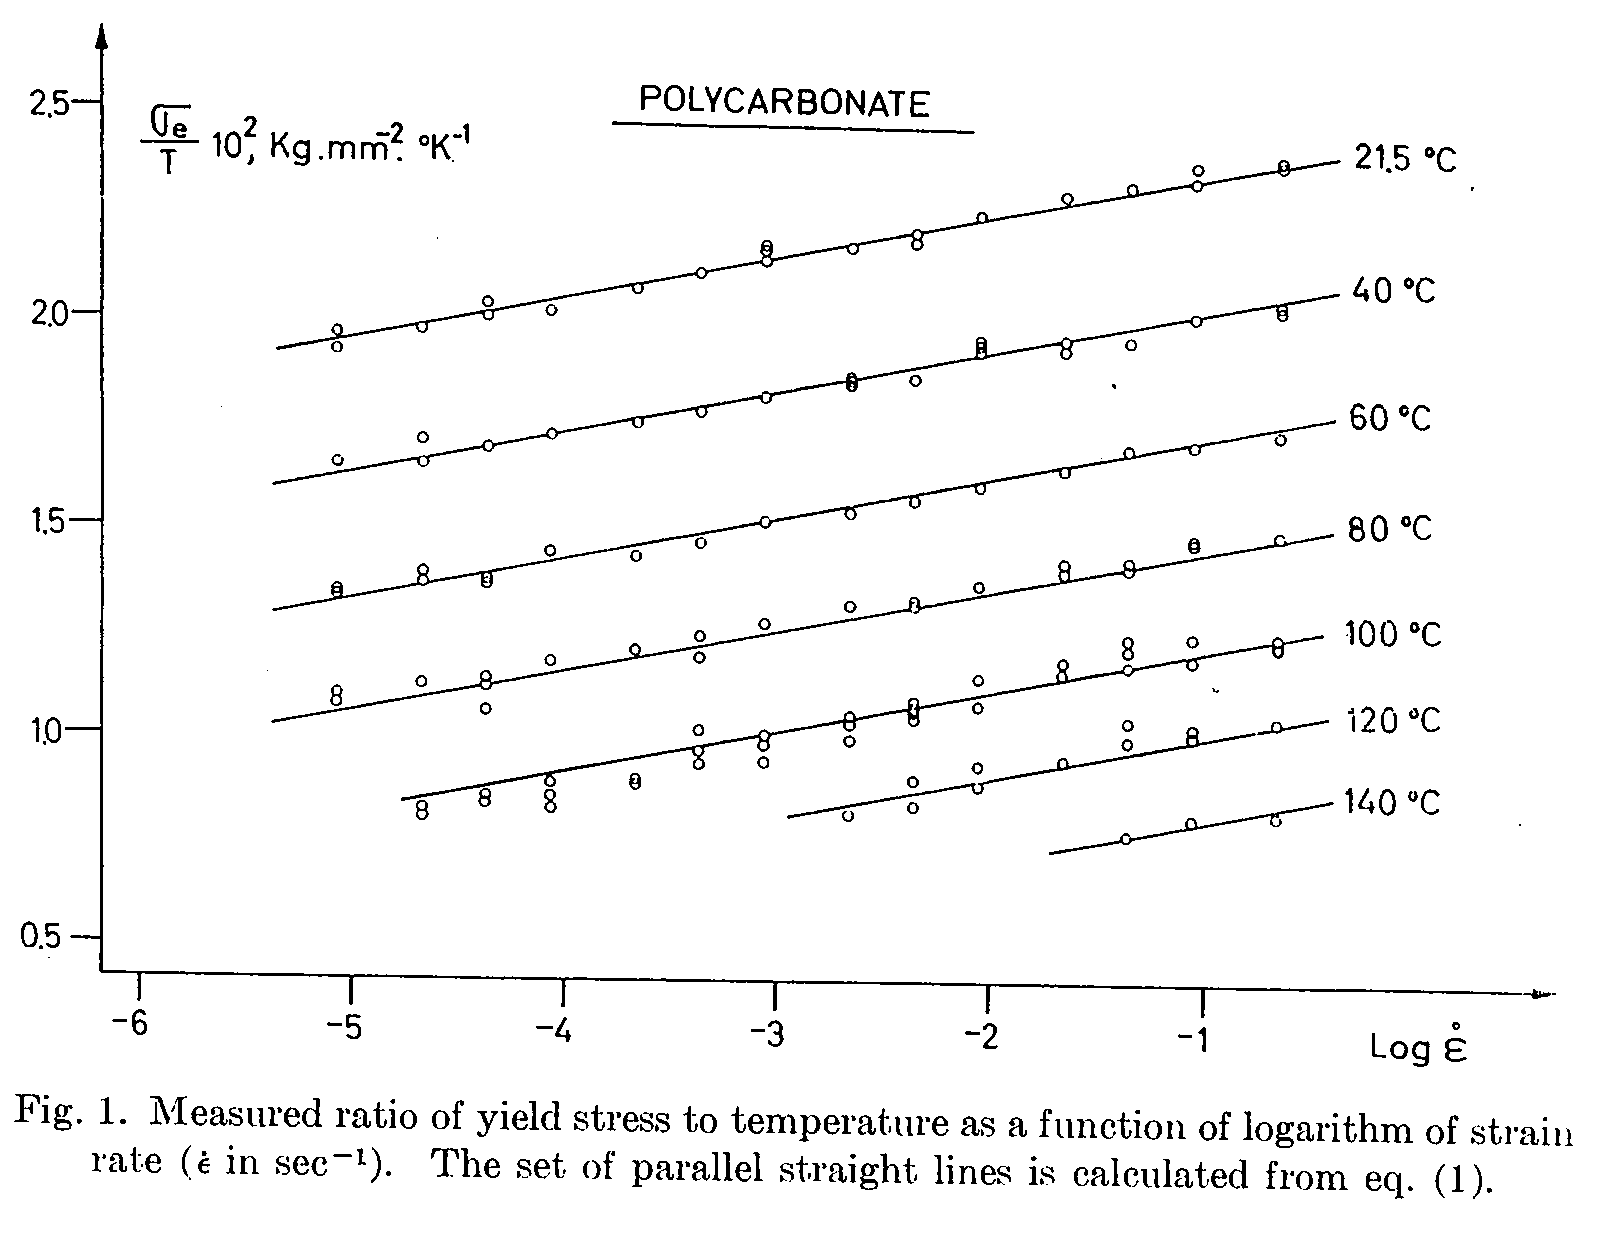
\includegraphics[width=\textwidth]{fig2.png}
% 	    \caption{Trajectry of Mean Square Internal Distance distribution of strands for 4-Chain Model}
% 	    \label{fig:e2e}
% 	\end{center}
% \end{minipage}
% \begin{minipage}{0.34\hsize}
% 	\begin{center}
% 		\includegraphics[width=\textwidth]{gt_comp_34.png}
%         \caption{Stress Relaxations for Uni-axial Step Strain($\lambda=2$)}
%         \label{fig:stress_rel}
% 	\end{center}
% \end{minipage}
% \begin{minipage}{0.32\hsize}
% 	\begin{center}
% 		\includegraphics[width=.8\textwidth]{N48_f4_PPA.png}
%         \caption{Primitive Path Analysis (PPA) for 4-Chain Model}
%         \label{fig:ppa}
% 	\end{center}
% \end{minipage}
% \end{figure}

\begin{figure}[htb]

    \begin{center}
        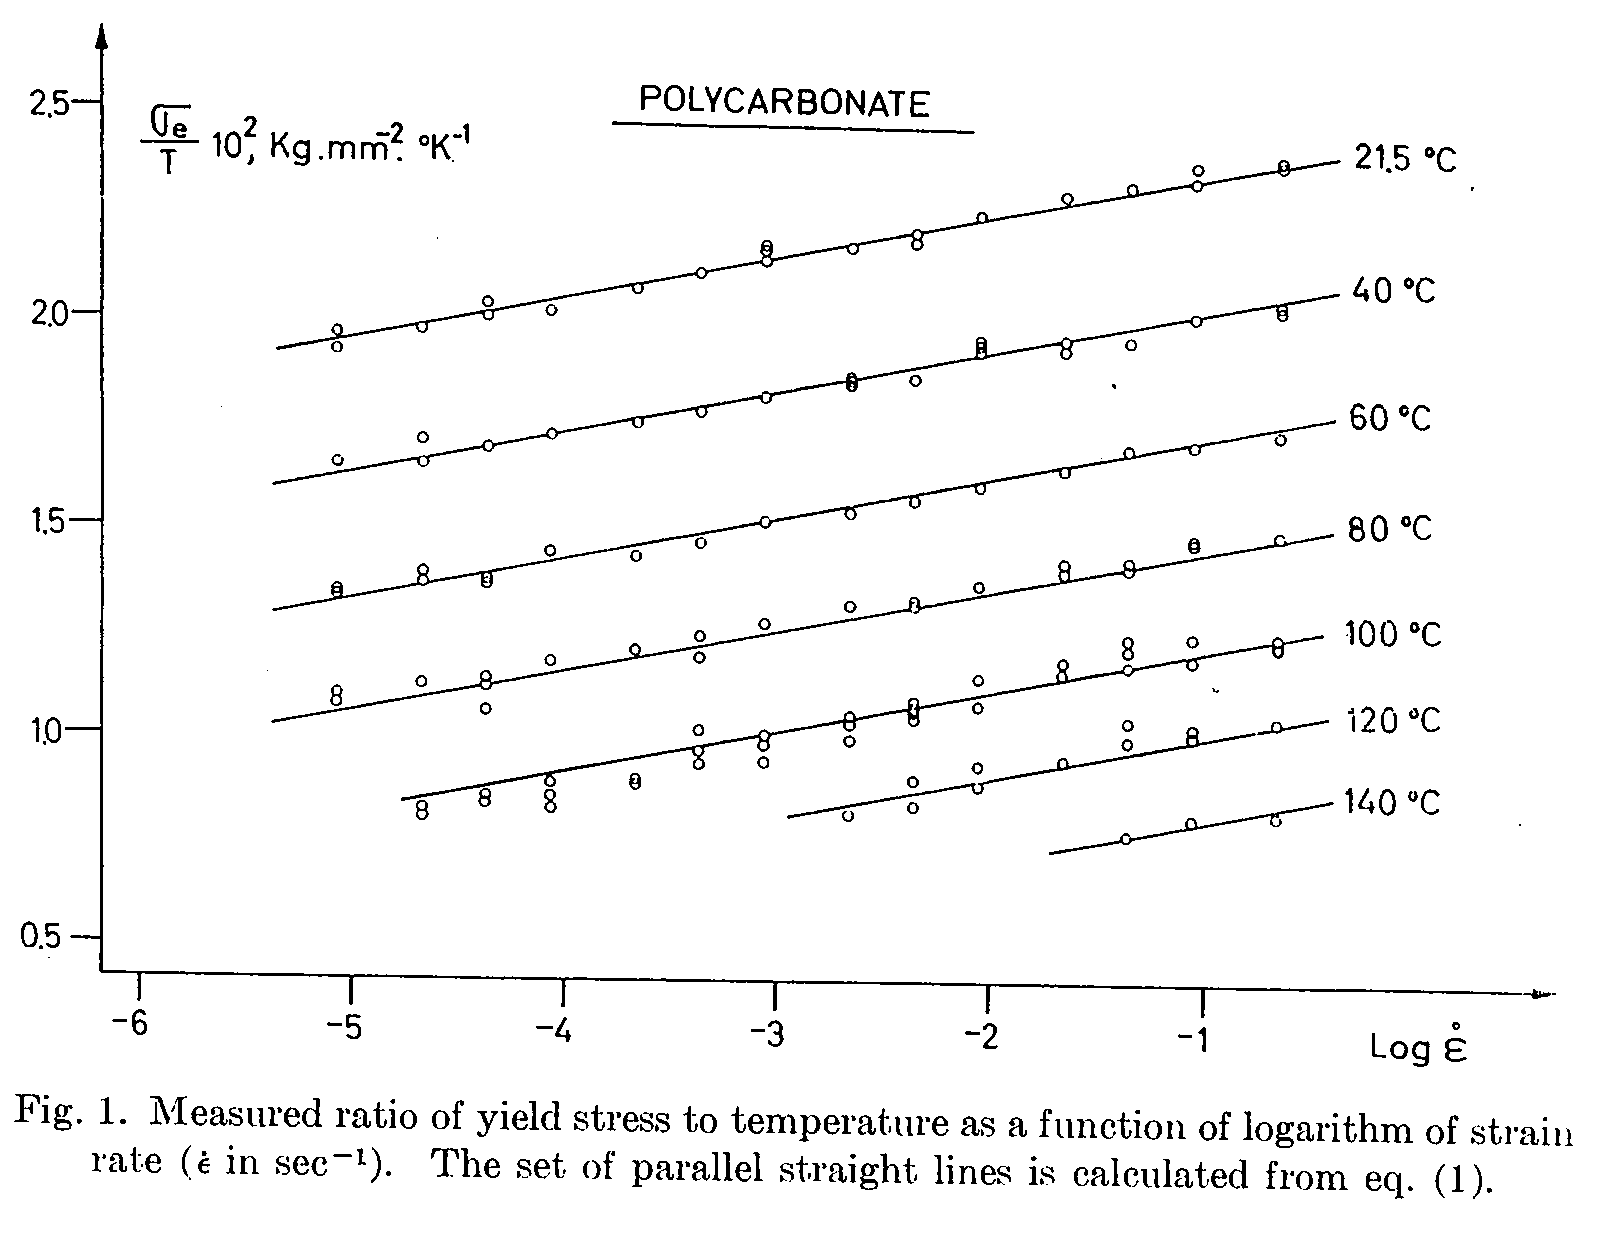
\includegraphics[width=.8\textwidth]{fig2.png}
	    \caption{Copied from ref.1}
	    \label{fig2}
	\end{center}
\end{figure}

\end{document}